\section{Additional technologies used in selection}
\label{ref:sel:tech}


% \section{Muon PID}
% \label{ref:selection:mu-pid}

% It is reported from previous analyses
% (\cite{PhysRevLett.115.111803,LHCb-ANA-2020-056}) that a tighter \muon PID
% requirement was very helpful in reducing \muon misidentification
% backgrounds\footnote{
%     This means a charged particle of other species is misidentified as a \muon.
%     For more details, see
%     \cref{ref:data-driven-templates:mu-misid:unfold-fake-mu}.
% }.
% To maintain minimum bias on \muon \pt, a multivariate BDT,
% referred as \UBDT, using uBDT method in TMVA class,
% is trained to reject misidentified \muon while keeping rejection
% efficiency flat on \pt,
% as described in \cite{LHCb-ANA-2020-056}.

% The \UBDT has been re-trained on LHCb run 2 MC\footnote{
%     The updated project can be found at
%     \techurllink{https://github.com/umd-lhcb/MuonBDTPid}{github/umd-lhcb/MuonBDTPid}.
% }.
% There is ongoing effort to study its efficiency against standard run 2 PID
% variables.
% Early report suggests the flatness on \pt is maintained while rejection
% efficiencies relative to existing PID cut are high for all but proton ($p$),
% as shown in \cref{fig:ubdt-eff}.

% % Generated with:
% %   https://github.com/umd-lhcb/pidcalib2, branch efficiency_study
% % first, run efficiency_gen/rdx-run2-ubdt-misidgen.sh
% % then, go inside scripts folder, run ./plots.py
% \begin{figure}[htb]
%     \centering
%     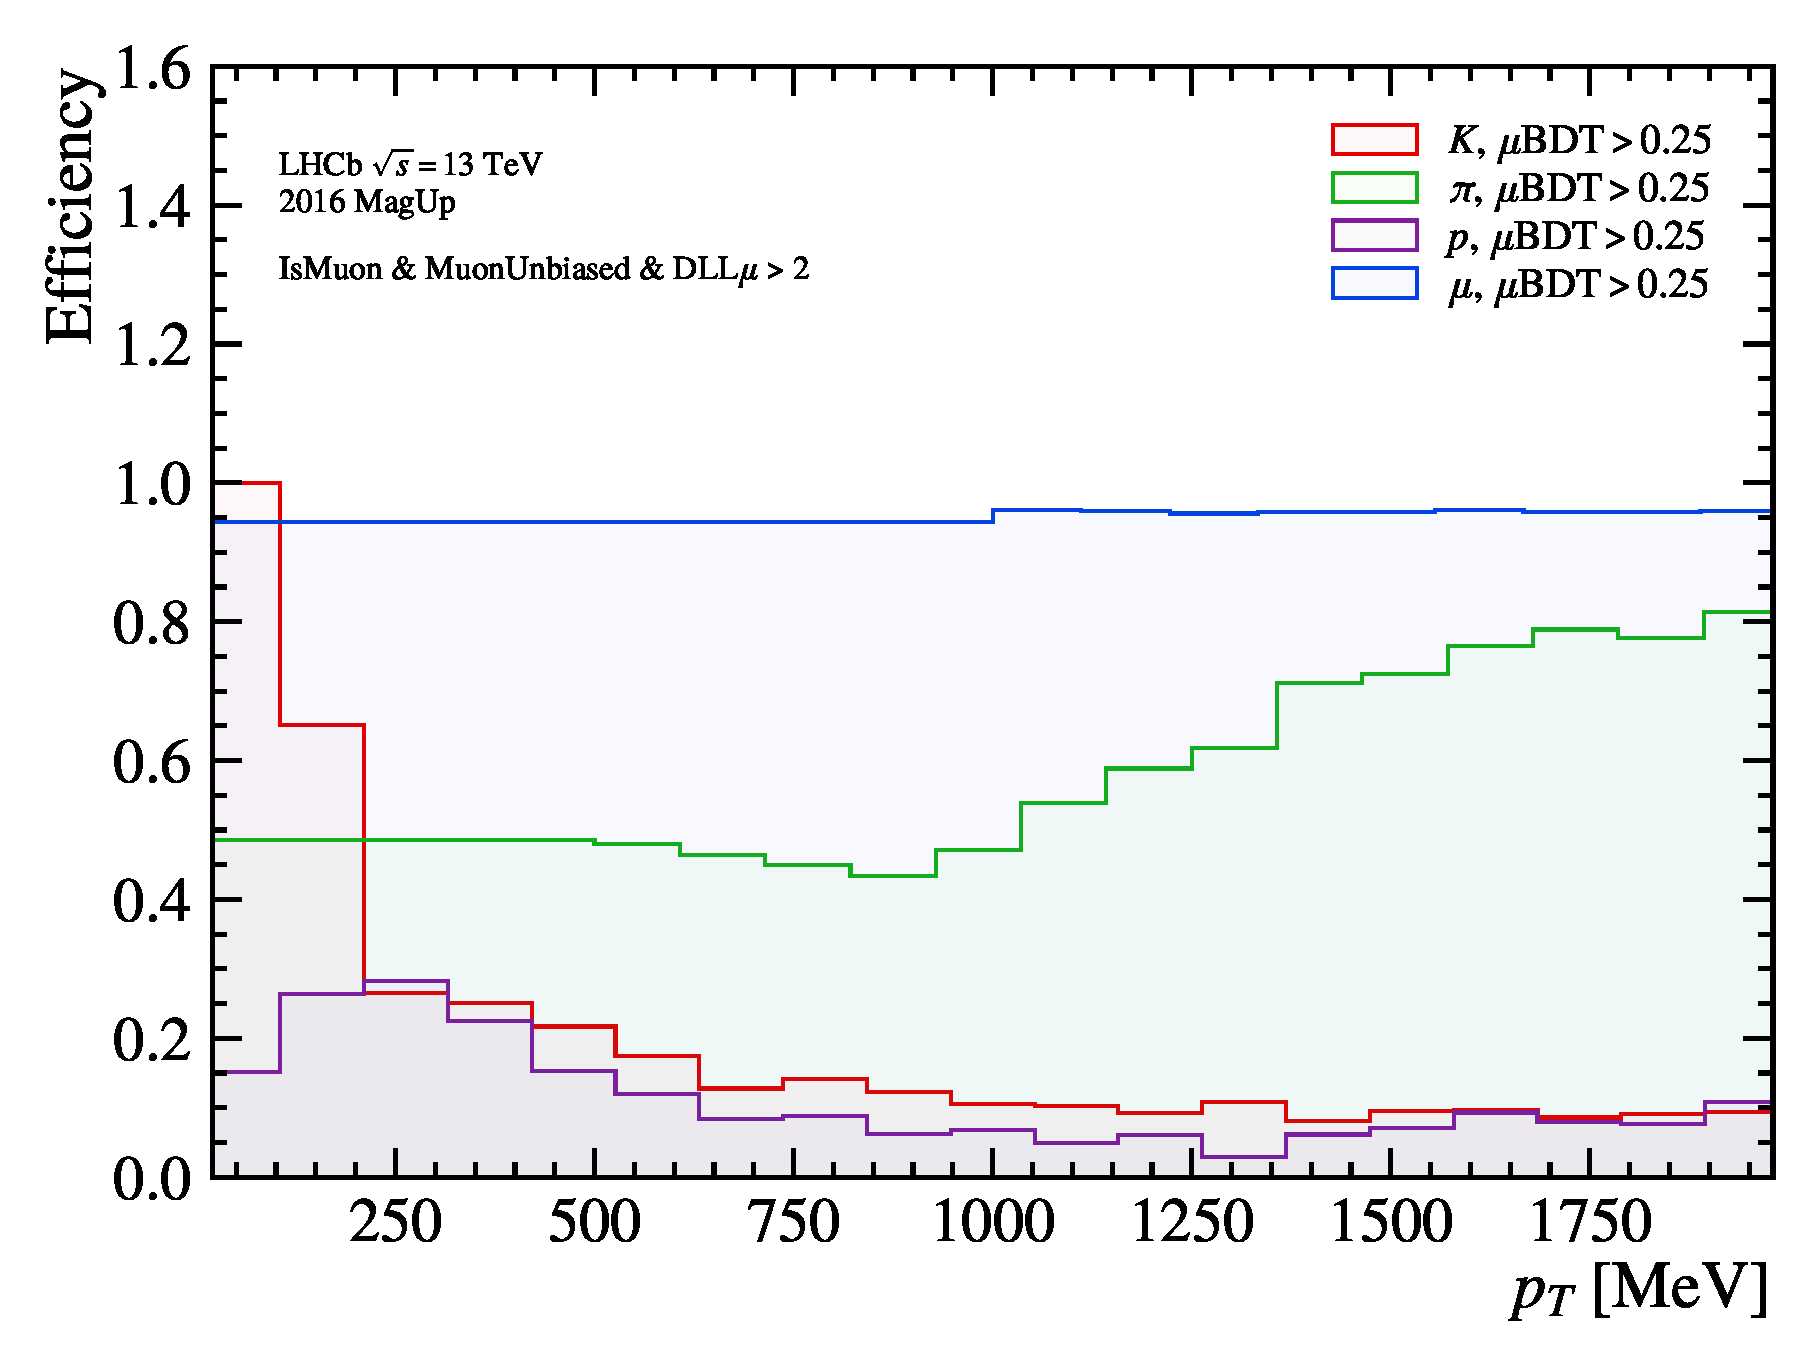
\includegraphics[width=0.45\textwidth]{./figs-selection/eff_Brunel_PT_up_pidcalib_ubdt_eff.pdf}
%     \hspace{1em}
%     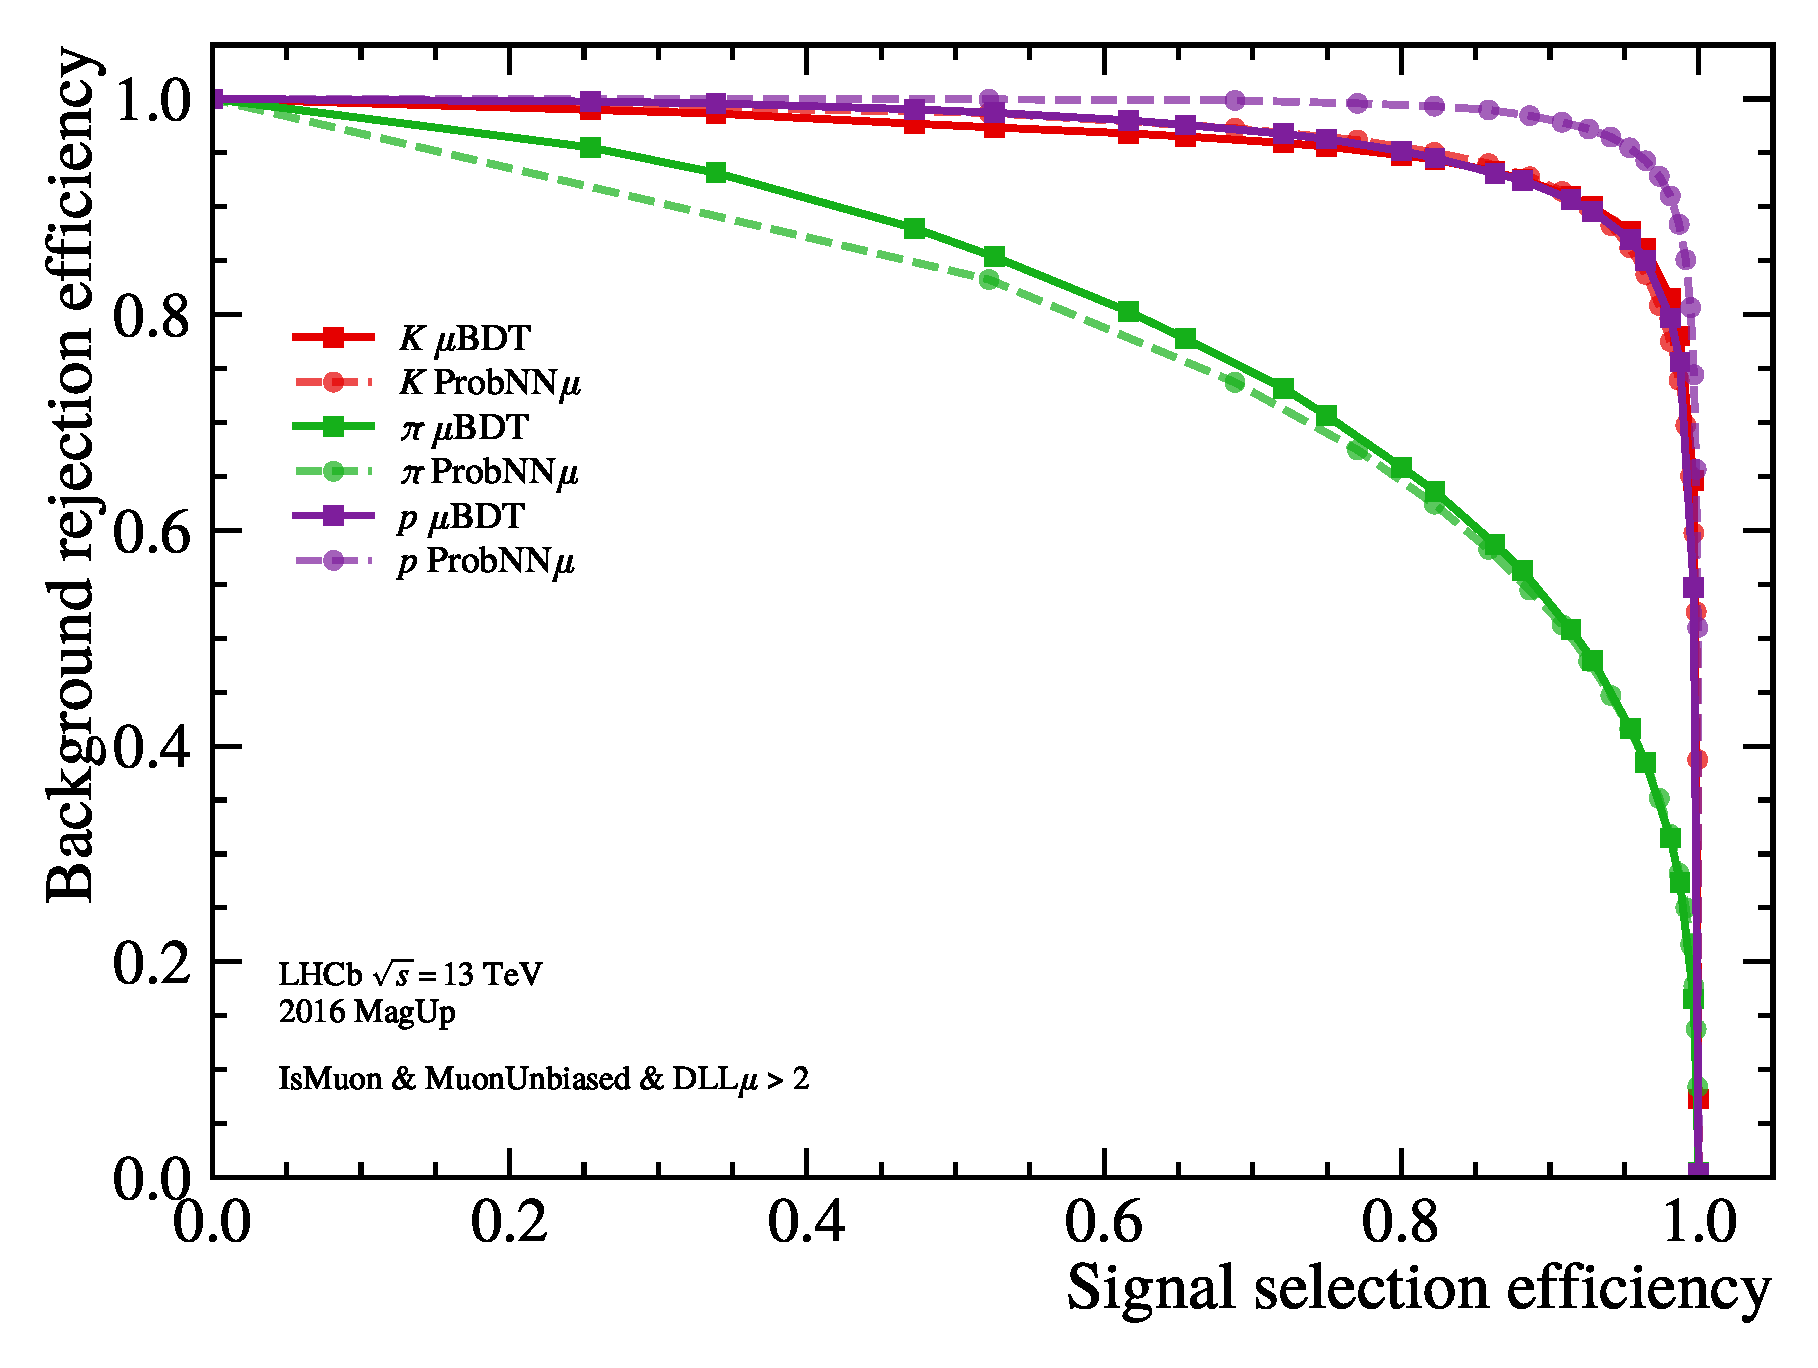
\includegraphics[width=0.45\textwidth]{./figs-selection/rej_v_eff_unbiased_Brunel_PT.pdf}

%     \caption{
%         Preliminary \UBDT study.
%         Left: \UBDT \muon selection efficiency is flat in \pt, with
%         global cut \isMuon \& $\text{\PID{\muon}}\! > 2$,
%         and $\UBDT > 0.25$.
%         Right: with the same global cut, \UBDT is more effective in rejecting
%         \pion than LHCb official \ProbNN{\muon}.
%         The \kaon rejection efficiencies are similar between the two;
%         the $p$ rejection efficiency is lower for \UBDT, but the absolute
%         rejection efficiency is high enough.
%     }
%     \label{fig:ubdt-eff}
% \end{figure}


% \section{Selected signal (ISO) and control (1OS, 2OS, DD) samples}
% \label{ref:selection:skims}

% The signal and control samples are selected by inspecting if there exists
% additional charged tracks that are compatible with coming from the
% reconstructed \B vertex.
% To predict the possibility of a charged track originating from the \B vertex,
% a multivariate BDT, referred as ``isolation BDT'', is used.
% The BDT is conceptually identical to the one used in
% \cite{LHCb-ANA-2020-056} but with the BDT re-trained based on LHCb run 2
% simulation.

% The isolation BDT\footnote{
%     The isolation BDT can be found at
%     \techurllink{https://github.com/umd-lhcb/TupleToolSemiLeptonic/blob/master/Phys/TupleToolSemiLeptonic/src/TupleToolApplyIsolation.cpp}{github/umd-lhcb/TupleToolSemiLeptonic}.
% } is added to the \davinci reconstruction sequence.
% It loops over all charged tracks in the event\footnote{
%     More specifically, these tracks are coming from
%     \texttt{StdAllNoPIDsPions}, \texttt{StdNoPIDsUpPions},
%     and \texttt{StdNoPIDsVeloPions}.
% },
% providing isolation scores for each of them where
% higher score implies higher probability of coming from the vertex, named as
% ``anti-isolated''.
% Three tracks with highest isolation scores\footnote{
%     The ones that are most likely to be anti-isolated.
% } are saved in the output file, in descending order\footnote{
%     So the first one is the most anti-isolated one among all charged tracks
%     in the event.
% }.

% Below a brief description for the signal sample and the main physics background
% control samples is provided.
% The actual isolation selections are listed in \cref{tab:skim-cut}.

% \begin{itemize}
%     \item ISO: $B \rightarrow D^{(*)} \lepton \neulb$, with $\lepton \in \{\muon,
%         \tauon\}$.
%         This is referred as signal, or ``isolated'', sample.
%         It requires that no additional charged track is from the \B vertex
%         (in a probabilistic sense, with probability related to the isolation
%         score)
%         and is compatible with a fully reconstructed \B decay
%         (ignoring missing neutrino(s)).

%     \item DD: $B \rightarrow D^{(*)}D X$,
%         with dominate $D \rightarrow \Kp \mun \neumb X$ sub-decays.
%         This is a double-charm ($DD$) control sample,
%         which is selected by requiring at least one anti-isolated track,
%         a \kaon-like long track\footnote{
%             This means the track went through both upstream and downstream
%             trackers, and is generally of good tracking quality.
%         } and a hard track in the three most anti-isolated tracks\footnote{
%             Note that these three requirements can be satisfied by a single
%             track.
%         }.

%     \item 1OS: $B \rightarrow D^{**} \lepton \neulb$.
%         This control sample, enriched in excited charm states,
%         requires one and only one additional anti-isolated charged long track
%         that is compatible with a \pion PID hypothesis and has correct charge
%         for a $D^{**} \rightarrow D^{(*+)}\pim$ decay.

%     \item 2OS: $B \rightarrow D^{**}_H \lepton \neulb$,
%         where $H$ stands for ``heavy''.
%         This control sample is enriched in highly excited (heavy) charm states,
%         which is selected by requiring two and only two anti-isolated \pion-like
%         long tracks of opposite charge,
%         capable of $D^{**}_H \rightarrow D^{(*)} \pip\pim$ decay.

%         % Why?
%         This sample also provides an independent selection of
%         $B \rightarrow D^{(*)}D X$ backgrounds, where the \pip\pim fit into the
%         $X$ category and \kaon escapes isolation detection.
% \end{itemize}

% \begin{table}[htb]
%     \caption{Signal and control sample isolation requirements.}
%     \label{tab:skim-cut}
%     \centering
%     \begin{tabular}{c|rll}
%         \toprule
%         {\bf Sample}  & {\bf Variable}              & {\bf Cuts}     \\
%         \midrule
%         ISO           & \isoBDT{1}                  & $< 0.15$       \\
%         \midrule
%         1OS           & \isoBDT{1}                  & $> 0.15$       \\
%                       & \isoBDT{2}                  & $< 0.15$       \\
%                       & \isoTrack{1}                & $= 3$\parnote{
%                           This means a long track.
%                       }                                              \\
%                       & $p_1$                       & $> 5$ GeV      \\
%                       & $p_{T,1}$                   & $> 0.15$ GeV   \\
%                       & \ProbNN{$K_1$}              & $< 0.2$        \\
%                       & $Q_1 \cdot \text{PID}_\Dz$\parnote{
%                           Apply to \Dz channel,
%                           which implies that the anti-isolated \pip can
%                           form a \Dstarp with the \Dz.
%                       }                             & $> 0$          \\
%                       & $Q_1 \cdot \text{PID}_\Dstar$\parnote{
%                           Apply to \Dstar channel.
%                           Here it is required that the anti-isolated \pim can
%                           form a $D^{**0}$ with the \Dstarp.
%                       }                             & $< 0$          \\
%         \midrule
%         2OS           & \isoBDT{1}                  & $> 0.15$       \\
%                       & \isoBDT{2}                  & $> 0.15$       \\
%                       & \isoBDT{3}                  & $< 0.15$       \\
%                       & \isoTrack{1}                & $= 3$          \\
%                       & \isoTrack{2}                & $= 3$          \\
%                       & {\footnotesize
%                          Max$(p_1 \cdot (p_{T,1} > 0.15 \text{ GeV}),
%                               p_2 \cdot (p_{T,2} > 0.15 \text{ GeV}))$
%                         }
%                                                     & $> 5$ GeV      \\
%                       & \ProbNN{$K_1$}              & $< 0.2$        \\
%                       & \ProbNN{$K_2$}              & $< 0.2$        \\
%                       & $Q_1 \cdot Q_2$             & $< 0$          \\
%         \midrule
%         DD            & \isoBDT{1}                  & $> 0.15$       \\
%                       & {\footnotesize$\begin{aligned}
%                             \text{Max}(
%                             &p_1 \cdot (p_{T,1} > 0.15\text{ GeV}),  \\
%                             &p_2 \cdot (p_{T,2} > 0.15\text{ GeV})
%                                  \cdot (\text{\isoBDT{2}} > -1.1),   \\
%                             &p_3 \cdot (p_{T,3} > 0.15\text{ GeV})
%                                  \cdot (\text{\isoBDT{3}} > -1.1)
%                             )
%                         \end{aligned}$}             & $> 5$ GeV      \\
%                       & Max(\ProbNN{$K_{1,2,3}$})   & $> 0.2$        \\
%                       & \isoTrack{\text{the one passing $K$ PID requirement}}
%                                                     & $= 3$          \\
%                       & \isoBDT{\text{the one passing $K$ PID requirement}}
%                                                     & $> -1.1$       \\
%         \bottomrule
%     \end{tabular}
%     \begin{flushleft}
%         \parnotes
%     \end{flushleft}
% \end{table}


\subsection{Veto of overlapping candidates}
\label{ref:se:tech:veto}

% See this note: https://github.com/umd-lhcb/rdx-run2-analysis/blob/master/docs/cuts/Dst_veto_in_D0.md
% TODO: The number need to be updated
Since the selection of a \Dstar\muon pair always requires the existence
of a \Dz\muon pair,
there is about 35\% of events in the signal sample\footnote{
    Defined in \cref{ref:sel:data:iso}.
} of the \Dstar channel leaks into \Dz channel.
This is likely due to the fact that slow \pion typically has poor tracking
resolution (small \ipChiSq), making the \Dz\pion vertex of poor quality which
makes the reconstruction fail and \Dstar partially reconstructed as \Dz.
To make \Dstar and \Dz channel more orthgonoal

To veto the overlapping candidates between \Dz and \Dstar channel,
a tool\footnote{
    Named \texttt{TupleToolApplyIsolationVetoDst}, which can be found at
    \techurllink{https://github.com/umd-lhcb/TupleToolSemiLeptonic/blob/master/Phys/TupleToolSemiLeptonic/src/TupleToolApplyIsolationVetoDst.cpp}{github/umd-lhcb/TupleToolSemiLeptonic}
}.
is added to the \davinci reconstruction sequence, which processes all tracks
in the event with the following procedure:

\begin{enumerate}
    \item Denote the track as $t$
    \item Refit a vertex from \Dz and $t$.
    \item Compute $\Delta m_\text{veto} \equiv m_{\Dz t} - m_\Dz$
    \item Test if $\Delta m_\text{veto} \in [140~\text{GeV}, 160~\text{GeV}]$.
        If it is, record $\Delta m_\text{veto}$ and the isolation BDT
        score of this track.
\end{enumerate}

From all recorded BDT scores and $\Delta m_\text{veto}$, the
$\Delta m_\text{veto}$ of the tracks with top two BDT scores are saved.
It is then filtered offline (listed in \cref{tab:offline-cut-d0})
that these two tracks,
the best slow \pion candidates,
are \emph{incompatible} with
forming a \Dz\pion vertex with a mass close to \Dstar PDG mass.

Note that this tool does not rank tracks based \emph{solely} on the isolation,
because the poor tracking resolution of the slow \pion implies that the track is
\emph{not guaranteed} to have a large isolation score, as it maybe more
compatible to be originating from PV, instead of the \B vertex.
Ranking tracks that fall within the $[140~\text{GeV}, 160~\text{GeV}]$
mass window based on their BDT scores
makes the veto procedure more robust, as reported in \cite{LHCb-ANA-2020-056}.

In addition, an alternative mass hypothesis is tested
(offline, also listed in \cref{tab:offline-cut-d0}), where the reconstructed
\muon is treated as a \pion,
and $\Delta m_\text{alt hypo} = m_{\Dz\muon_\text{as \pion}} - m_\Dz$
is computed\footnote{
    By using the 3-momentum of the \muon, while using $m_\pion$ as the invariant
    mass of the track.
} and required to be inconsistent with \Dstar PDG mass.

The veto procedures are applied on all samples of the \Dz channel only.
